% Espacio de estados — forma general: x' = Ax + Bu,  y = Cx + Du
\documentclass[border=6pt]{standalone}
\usepackage{amsmath}
\usepackage{tikz}
\usetikzlibrary{arrows.meta, calc}
\begin{document}
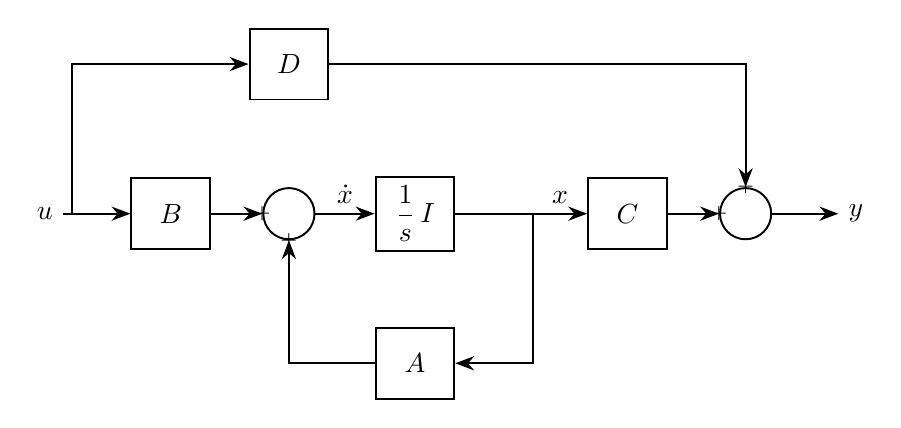
\begin{tikzpicture}[
  >={Stealth[length=2.4mm]}, line width=0.7pt,
  block/.style={draw, minimum width=1.0cm, minimum height=0.9cm},
  sum/.style={draw, circle, minimum size=6.5mm, inner sep=0pt}]

  % cadena principal
  \node (u)   at (0,0)    {$u$};
  \node[block] (B)  at (1.6,0)  {$B$};
  \node[sum]   (s1) at (3.1,0)  {};
  \node[block] (I)  at (4.7,0)  {$\dfrac{1}{s}\,I$};
  \coordinate (bx) at (6.2,0);
  \node[block] (C)  at (7.4,0)  {$C$};
  \node[sum]   (s2) at (8.9,0)  {};
  \node (y)   at (10.3,0)  {$y$};

  \draw[->] (u)  -- (B);
  \draw[->] (B)  -- (s1);
  \draw[->] (s1) -- (I) node[midway, above]{$\dot{x}$};
  \draw[-]  (I)  -- (bx);
  \draw[->] (bx) -- (C) node[midway, above]{$x$};
  \draw[->] (C)  -- (s2);
  \draw[->] (s2) -- (y);

  % realimentación de estado A
  \node[block] (A) at (4.7,-1.9) {$A$};
  \draw[->] (bx) |- (A);
  \draw[->] (A) -| (s1);
  \node at ($(s1)+(0.0,-0.34)$) {\scriptsize$+$};

  % feedforward D
  \node[block] (D) at (3.1,1.9) {$D$};
  \draw[->] ($(u)+(0.35,0)$) |- (D);
  \draw[->] (D) -| (s2);
  \node at ($(s2)+(0.0,0.34)$) {\scriptsize$+$};
  \node at ($(s2)+(-0.34,0.0)$) {\scriptsize$+$};

  % signos del sumador de estado
  \node at ($(s1)+(-0.34,0.0)$) {\scriptsize$+$};
\end{tikzpicture}
\end{document}
